% Options for packages loaded elsewhere
\PassOptionsToPackage{unicode}{hyperref}
\PassOptionsToPackage{hyphens}{url}
%
\documentclass[
]{book}
\usepackage{lmodern}
\usepackage{amssymb,amsmath}
\usepackage{ifxetex,ifluatex}
\ifnum 0\ifxetex 1\fi\ifluatex 1\fi=0 % if pdftex
  \usepackage[T1]{fontenc}
  \usepackage[utf8]{inputenc}
  \usepackage{textcomp} % provide euro and other symbols
\else % if luatex or xetex
  \usepackage{unicode-math}
  \defaultfontfeatures{Scale=MatchLowercase}
  \defaultfontfeatures[\rmfamily]{Ligatures=TeX,Scale=1}
\fi
% Use upquote if available, for straight quotes in verbatim environments
\IfFileExists{upquote.sty}{\usepackage{upquote}}{}
\IfFileExists{microtype.sty}{% use microtype if available
  \usepackage[]{microtype}
  \UseMicrotypeSet[protrusion]{basicmath} % disable protrusion for tt fonts
}{}
\makeatletter
\@ifundefined{KOMAClassName}{% if non-KOMA class
  \IfFileExists{parskip.sty}{%
    \usepackage{parskip}
  }{% else
    \setlength{\parindent}{0pt}
    \setlength{\parskip}{6pt plus 2pt minus 1pt}}
}{% if KOMA class
  \KOMAoptions{parskip=half}}
\makeatother
\usepackage{xcolor}
\IfFileExists{xurl.sty}{\usepackage{xurl}}{} % add URL line breaks if available
\IfFileExists{bookmark.sty}{\usepackage{bookmark}}{\usepackage{hyperref}}
\hypersetup{
  pdftitle={Introdução ao R para análise de dados e construção de gráficos},
  pdfauthor={Alessandro Samuel-Rosa},
  hidelinks,
  pdfcreator={LaTeX via pandoc}}
\urlstyle{same} % disable monospaced font for URLs
\usepackage{color}
\usepackage{fancyvrb}
\newcommand{\VerbBar}{|}
\newcommand{\VERB}{\Verb[commandchars=\\\{\}]}
\DefineVerbatimEnvironment{Highlighting}{Verbatim}{commandchars=\\\{\}}
% Add ',fontsize=\small' for more characters per line
\usepackage{framed}
\definecolor{shadecolor}{RGB}{248,248,248}
\newenvironment{Shaded}{\begin{snugshade}}{\end{snugshade}}
\newcommand{\AlertTok}[1]{\textcolor[rgb]{0.94,0.16,0.16}{#1}}
\newcommand{\AnnotationTok}[1]{\textcolor[rgb]{0.56,0.35,0.01}{\textbf{\textit{#1}}}}
\newcommand{\AttributeTok}[1]{\textcolor[rgb]{0.77,0.63,0.00}{#1}}
\newcommand{\BaseNTok}[1]{\textcolor[rgb]{0.00,0.00,0.81}{#1}}
\newcommand{\BuiltInTok}[1]{#1}
\newcommand{\CharTok}[1]{\textcolor[rgb]{0.31,0.60,0.02}{#1}}
\newcommand{\CommentTok}[1]{\textcolor[rgb]{0.56,0.35,0.01}{\textit{#1}}}
\newcommand{\CommentVarTok}[1]{\textcolor[rgb]{0.56,0.35,0.01}{\textbf{\textit{#1}}}}
\newcommand{\ConstantTok}[1]{\textcolor[rgb]{0.00,0.00,0.00}{#1}}
\newcommand{\ControlFlowTok}[1]{\textcolor[rgb]{0.13,0.29,0.53}{\textbf{#1}}}
\newcommand{\DataTypeTok}[1]{\textcolor[rgb]{0.13,0.29,0.53}{#1}}
\newcommand{\DecValTok}[1]{\textcolor[rgb]{0.00,0.00,0.81}{#1}}
\newcommand{\DocumentationTok}[1]{\textcolor[rgb]{0.56,0.35,0.01}{\textbf{\textit{#1}}}}
\newcommand{\ErrorTok}[1]{\textcolor[rgb]{0.64,0.00,0.00}{\textbf{#1}}}
\newcommand{\ExtensionTok}[1]{#1}
\newcommand{\FloatTok}[1]{\textcolor[rgb]{0.00,0.00,0.81}{#1}}
\newcommand{\FunctionTok}[1]{\textcolor[rgb]{0.00,0.00,0.00}{#1}}
\newcommand{\ImportTok}[1]{#1}
\newcommand{\InformationTok}[1]{\textcolor[rgb]{0.56,0.35,0.01}{\textbf{\textit{#1}}}}
\newcommand{\KeywordTok}[1]{\textcolor[rgb]{0.13,0.29,0.53}{\textbf{#1}}}
\newcommand{\NormalTok}[1]{#1}
\newcommand{\OperatorTok}[1]{\textcolor[rgb]{0.81,0.36,0.00}{\textbf{#1}}}
\newcommand{\OtherTok}[1]{\textcolor[rgb]{0.56,0.35,0.01}{#1}}
\newcommand{\PreprocessorTok}[1]{\textcolor[rgb]{0.56,0.35,0.01}{\textit{#1}}}
\newcommand{\RegionMarkerTok}[1]{#1}
\newcommand{\SpecialCharTok}[1]{\textcolor[rgb]{0.00,0.00,0.00}{#1}}
\newcommand{\SpecialStringTok}[1]{\textcolor[rgb]{0.31,0.60,0.02}{#1}}
\newcommand{\StringTok}[1]{\textcolor[rgb]{0.31,0.60,0.02}{#1}}
\newcommand{\VariableTok}[1]{\textcolor[rgb]{0.00,0.00,0.00}{#1}}
\newcommand{\VerbatimStringTok}[1]{\textcolor[rgb]{0.31,0.60,0.02}{#1}}
\newcommand{\WarningTok}[1]{\textcolor[rgb]{0.56,0.35,0.01}{\textbf{\textit{#1}}}}
\usepackage{longtable,booktabs}
% Correct order of tables after \paragraph or \subparagraph
\usepackage{etoolbox}
\makeatletter
\patchcmd\longtable{\par}{\if@noskipsec\mbox{}\fi\par}{}{}
\makeatother
% Allow footnotes in longtable head/foot
\IfFileExists{footnotehyper.sty}{\usepackage{footnotehyper}}{\usepackage{footnote}}
\makesavenoteenv{longtable}
\usepackage{graphicx,grffile}
\makeatletter
\def\maxwidth{\ifdim\Gin@nat@width>\linewidth\linewidth\else\Gin@nat@width\fi}
\def\maxheight{\ifdim\Gin@nat@height>\textheight\textheight\else\Gin@nat@height\fi}
\makeatother
% Scale images if necessary, so that they will not overflow the page
% margins by default, and it is still possible to overwrite the defaults
% using explicit options in \includegraphics[width, height, ...]{}
\setkeys{Gin}{width=\maxwidth,height=\maxheight,keepaspectratio}
% Set default figure placement to htbp
\makeatletter
\def\fps@figure{htbp}
\makeatother
\setlength{\emergencystretch}{3em} % prevent overfull lines
\providecommand{\tightlist}{%
  \setlength{\itemsep}{0pt}\setlength{\parskip}{0pt}}
\setcounter{secnumdepth}{5}
\usepackage{booktabs}
\usepackage[]{natbib}
\bibliographystyle{apalike}

\title{Introdução ao R para análise de dados e construção de gráficos}
\author{Alessandro Samuel-Rosa}
\date{2020-11-23}

\begin{document}
\maketitle

{
\setcounter{tocdepth}{1}
\tableofcontents
}
\hypertarget{apresentauxe7uxe3o}{%
\chapter{Apresentação}\label{apresentauxe7uxe3o}}

\hypertarget{r-rstudio}{%
\chapter{R \& RStudio}\label{r-rstudio}}

A página do projeto R na Internet pode ser acessada pelo endereço \url{https://www.r-project.org/}. Nela você encontra grande quantidade de informação sobre o R. Estão disponíveis diversos manuais de uso (\emph{Documentation} \textgreater{} \emph{Manuals}), bem como livros (\emph{Documentation} \textgreater{} \emph{Books}) e artigos publicados na revista do projeto (\emph{Documentation} \textgreater{} \emph{The R Journal}). Também há uma página com respostas às perguntas mais frequentes (\emph{Documentation} \textgreater{} \emph{FAQs}) e uma página inteira explicando como é possível conseguir ajuda sozinho antes de recorrer a terceiros (\emph{Help With R} \textgreater{} \emph{Getting Help})\footnote{Como a documentação do R é extensa e a maioria dos colaboradores do projeto não são pagos pelo trabalho desenvolvido, recomendo que você sempre procure, primeiro, resolver qualquer dúvida sozinho.}.

O procedimento de instalação do R depende do sistema operacional (\href{https://en.wikipedia.org/wiki/Operating_system}{OS}, do inglês \emph{operating system}) de seu computador:

\begin{itemize}
\tightlist
\item
  Linux: \url{https://cloud.r-project.org/bin/linux/}
\item
  (Mac) OS X: \url{https://cloud.r-project.org/bin/macosx/}
\item
  Windows: \url{https://cloud.r-project.org/bin/windows/base/}
\end{itemize}

A página de cada OS possui as instruções necessárias para descarregar e instalar o R em seu computador. Em geral, o processo de instalação é muito parecido com aquele de outros programas de computador que você está acostumado a usar.

Depois de completada a instalação do R, é hora de instalar o RStudio. A última versão gratuíta\footnote{Licença AGPL v3.} do instalador do RStudio para o OS de seu computador pode ser descarregada do seguinte endereço na Internet:

\begin{itemize}
\tightlist
\item
  \url{https://www.rstudio.com/products/rstudio/download/}
\end{itemize}

Assim como para o R, você não encontrará maiores dificuldades no processo de instalação do RStudio.

Depois de instalados R e RStudio, inicie o RStudio em seu computador. A interface do RStudio deve se parecer mais ou menos com aquela mostrada na figura abaixo\footnote{A disposição dos painéis do ambiente de trabalho pode ser alterada acessando \emph{Tools} \textgreater{} \emph{Global Options} \textgreater{} \emph{Pane Layout}.}.

\begin{figure}
\centering
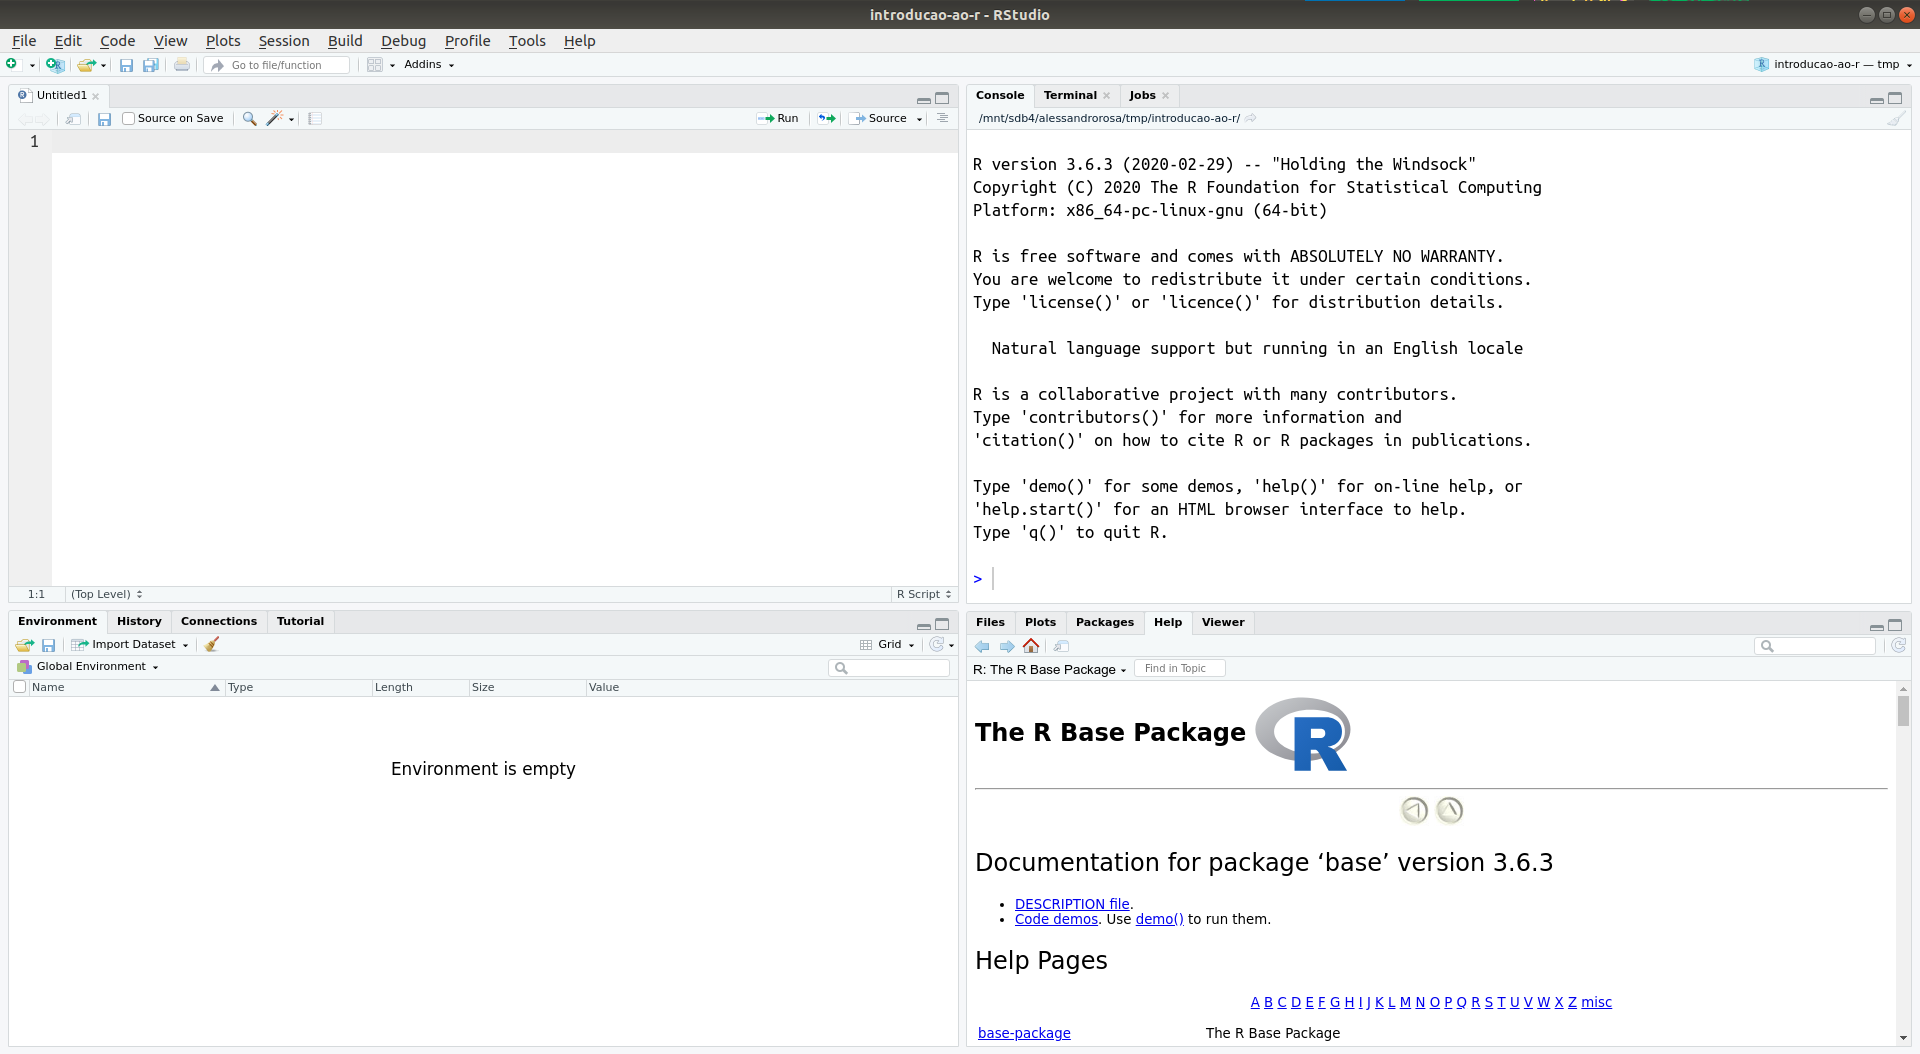
\includegraphics{img/rstudio.png}
\caption{RStudio: ambiente de desenvolvimento integrado (IDE) para R em sua versão para Linux.}
\end{figure}

O RStudio é composto por quatro painéis retangulares que ocupam seus quadrantes:

\begin{itemize}
\tightlist
\item
  Painel superior esquerdo: usado para preparar o roteiro (\emph{script}) de análise de dados.
\item
  Painel superior direito: interface de linha de comando (CLI), o console do R.
\item
  Painel inferior direito: serve à visualização de gráficos e páginas de ajuda do R.
\item
  Painel inferior esquerdo: apresenta informações sobre a sessão de trabalho.
\end{itemize}

Dentre os quatro painéis, é no painel superior esquerdo que passamos a maior parte do tempo quando analisamos dados no R. É ali que redigimos aquilo que queremos que o R faça com nossos dados na forma de comandos usando a linguagem do R. Para nos comunicamos com o R, enviamos esses comandos para o console do R, localizado no painel superior direito. Os resultados produzidos pelo R podem ser emitidos, tanto no console (tabelas), como no painel inferior direito (gráficos). Se não soubermos como nos comunicarmos com o R para que execute determinada função, podemos visitara aba de ajuda localizada no painel inferior direito.

\hypertarget{diretuxf3rio-de-arquivos}{%
\chapter{Diretório de arquivos}\label{diretuxf3rio-de-arquivos}}

Um dos passos mais importatantes de qualquer projeto é a criação de uma estrutura racional de diretórios de arquivos. Isso pode ser feito diretamente a partir do RStudio. Para isso, basta acessar \emph{File} \textgreater{} \emph{New Project\ldots{}} \textgreater{} \emph{New Directory} \textgreater{} \emph{New Project}. Na janela que abrir, são definidos o nome do diretório que armazenará os arquivos do projeto\footnote{Deve ser dada preferência a um nome curto e fácil de lembrar e relacionar com o escopo do projeto (mnemônico). Além disso, devem ser utilizadas apenas letras minúsculas e sem acentuação, substituindo os espaços por traços. Isso facilitará a gestão programática dos arquivos do projeto.} e o local do sistema de arquivos do computador onde esse diretório ficará localizado. Feito isso, o RStudio será reinicializado e o painel inferior direito (aba \emph{Files}) mostrará o interior do diretório que acabou de ser criado.

A seguinte estrutura de diretórios de arquivos deve ser criada no interior do diretório recém criado:

\begin{verbatim}
nome-do-projeto
|- code/
|- data/
|- docs/
|- res/
|  |- fig/
|  |- tab/
|- tmp/
|- README.md
\end{verbatim}

São cinco subdiretórios, cada um deles com o propósito de armazenar arquivos com conteúdos específicos:

\begin{itemize}
\tightlist
\item
  \texttt{code}: roteiros de análise de dados escritos usando a linguagem R.
\item
  \texttt{data}: dados das variáveis que serão estudadas no projeto.
\item
  \texttt{docs}: documentos de texto relacionados ao projeto.
\item
  \texttt{res}: resultados do projeto exportados como figuras e tabelas---figuras podem ser armazenadas no subdiretório \texttt{fig}, enquanto o subdiretório \texttt{tab} pode ser usado para armazenar tabelas.
\item
  \texttt{tmp}: arquivos temporários irrelevantes.
\end{itemize}

Diretórios podem ser criados diretamente no painel inferior direito do RStudio. Para isso, basta acessar \emph{New Folder} e definir o nome do diretório desejado conforme listado acima.

O próximo passo é criar um arquivo com a descrição do projeto. Isso é importante para garantir que, da próxima vez que você visitar esse diretório de arquivos, não tenha que depender inteiramente da sua memória. O arquivo \texttt{README.md} tem essa finalidade. Para criar esse arquivo, acesse \emph{File} \textgreater{} \emph{New File} e selecione a opção \emph{Markdown File}. O arquivo que abrir no painel superior esquerdo do RStudio deve ser salvo na raiz do diretório do projeto usando o nome \texttt{README.md} acessando \emph{File} \textgreater{} \emph{Save As\ldots{}}. Depois disso, registre no \texttt{README.md} informações essenciais do projeto como nome, equipe participante e data de início. O arquivo \texttt{README.md} também pode ser usado para descrever o conteúdo de cada um dos subdiretórios do projeto. Ao longo do desenvolvimento do projeto, ele será bastante útil para anotas as decisões tomadas e resumir os resultados alcançados.

Para concluir a construção da estrutura do diretório de arquivos, precisamos criar apenas mais um arquivo, agora no interior do diretório \texttt{code}. Esse arquivo será usado para redigir e armazenar o roteiro de análise de dados usando a linguagem R. Para criar esse arquivo, acesse \emph{File} \textgreater{} \emph{New File} e selecione a opção \emph{R Script}. Salve o arquivo que abrir no painel superior esquerdo do RStudio acessando \emph{File} \textgreater{} \emph{Save As\ldots{}}---você pode atribuir um nome curto como \texttt{main.R}.

\hypertarget{operauxe7uxf5es-matemuxe1ticas}{%
\chapter{Operações matemáticas}\label{operauxe7uxf5es-matemuxe1ticas}}

Vamos fazer algumas operações matemáticas para nos familiarizar com o R. Inicie copiando e colando a linha de comando abaixo no console do R localizado no painel superior direito do RStudio. Em seguida, pressione a tecla \emph{Enter}.

\begin{Shaded}
\begin{Highlighting}[]
\CommentTok{# Operações matemáticas no R: soma}
\DecValTok{2} \OperatorTok{+}\StringTok{ }\DecValTok{3}
\end{Highlighting}
\end{Shaded}

O console do R deve ter retornado o valor \texttt{5} como resultado da operação realizada. Agora realize a operação de subtração \texttt{2\ -\ 3}. O valor retornado pelo console do R deve ser \texttt{-1}\footnote{O espaçamento entre número e operador matemático não tem importância do ponto de vista da operação matemática. Contudo, do ponto de vista estético, para facilitar a leitura dos comandos, costuma-se usar a formatação com espaços \texttt{2\ +\ 3} em vez de \texttt{2+3}.}.

Os símbolos da linguagem R para realizar as operações matemáticas básicas são os mesmos encontrados em qualquer calculadora científica: \texttt{+} para adição, \texttt{*} para multiplização, \texttt{/} para divisão e \texttt{-} para subtração. São também os mesmos símbolos utilizados em planilhas eletrônicas de edição de dados. Isso significa que podemos deduzir algumas coisas sobre o funcionamento do R a partir daquilo que conhecemos de outras ferramentas dedicadas à análise e manipulação de dados.

\begin{center}\rule{0.5\linewidth}{0.5pt}\end{center}

\textbf{\emph{Tarefa:}} \emph{Realize todas as quatro operações matemáticas fundamentais utilizando diferentes valores para conhecer melhor o funcionamento básico do R. Registre essas operações no arquivo \texttt{main.R}, inserindo comentários textuais sobre cada uma delas.}

\begin{center}\rule{0.5\linewidth}{0.5pt}\end{center}

Um elemento importante presente no bloco acima é o comentário precedido pelo símbolo \texttt{\#} (cerquilha). Na linguagem R, a cerquilha tem o papel de indicar o início de um comentário textual que serve de instrução à pessoa que está escrevendo ou lendo o roteiro de análise do dados. Esses comentários podem ser incluídos, tanto em uma linha própria do roteiro, como na mesma linha após um comando, mas nunca antes de um comando. A inclusão de comentários textuais ao logo do roteiro serve para documentarmos a atividade que estamos realizando. Isso permite que outros, e nós mesmos, algumas semanas ou meses mais tarde, possamos entender o propósito de cada uma das linhas de comando redigidas.

O bloco abaixo apresenta mais algumas operações matemáticas.

\begin{Shaded}
\begin{Highlighting}[]
\DecValTok{2}\OperatorTok{^}\DecValTok{2}      \CommentTok{# Potenciação (ou exponenciação)}
\KeywordTok{log}\NormalTok{(}\DecValTok{4}\NormalTok{)   }\CommentTok{# Função logarítmica}
\KeywordTok{sqrt}\NormalTok{(}\DecValTok{25}\NormalTok{) }\CommentTok{# Raiz quadrada}
\end{Highlighting}
\end{Shaded}

As duas últimas operações apresentadas no bloco acima são representadas por identificadores, especificamente, as ``palavras'' \texttt{log} e \texttt{sqrt}, seguidas por dois parênteses contendo um valor numérico em seu interior. As expressões \texttt{log()} e \texttt{sqrt()} identificam funções do R, nesse caso, as funções logarítmica e raiz quadrada.

\begin{center}\rule{0.5\linewidth}{0.5pt}\end{center}

\textbf{\emph{Tarefa:}} \emph{Identifique as funções do R utilizadas para realizar as operações de soma, multiplicação e subtração. Registre essas funções no arquivo \texttt{main.R}, inserindo comentários textuais sobre cada uma delas.}

\hypertarget{funuxe7uxf5es-e-objetos}{%
\chapter{Funções e objetos}\label{funuxe7uxf5es-e-objetos}}

A gramática da linguagem R possui dois elementos principais: as palavras reservadas e as palavras-chave. As \textbf{\emph{palavras reservadas}} constituem signos com significado especial para a linguagem. Elas não podem ser utilizadas para outros fins que não aqueles especificados internamente no R. Algumas dessas palavras reservadas são \texttt{if}, \texttt{else}, \texttt{while}, \texttt{TRUE} e \texttt{FALSE}\footnote{O editor de comandos do RStudio destaca as palavras reservadas em azul para facilitar sua identificação. Busque pelo termo \emph{reserved} no painel de ajuda do RStudio para conhecer todas as palavras reservadas da linguagem R.}.

As \textbf{\emph{palavras-chave}} são aquelas utilizadas para identificar funções e objetos. \textbf{\emph{Funções}} nada mais são do que operações matemáticas e lógicas\footnote{Como diria John Chambers, tudo o que ``acontece'' no R acontece pela ação de uma função.}. Assim, as palavras-chave que identificam funções são aquelas que acionam tais operações. São elas que possibilitam, por exemplo, enviar ao R o comando para que realize determinada análise estatística de determinado conjunto de dados. A maioria das operações utilizadas na análise de dados já está definida na linguagem do R, como é o caso de \texttt{log}, \texttt{sqrt}, \texttt{sum}, \texttt{prod}, \texttt{diff}, \texttt{abs}, \texttt{cos}, \texttt{tan}, \texttt{det}, \texttt{exp}, \texttt{max}, \texttt{min}, \texttt{mean}, \texttt{median}, entre muitas outras.

\begin{center}\rule{0.5\linewidth}{0.5pt}\end{center}

\textbf{\emph{Tarefa:}} \emph{A aba de ajuda do RStudio possui, em seu canto superior direito, uma caixa de busca. Digite a primeira letra de seu nome e selecione, na lista suspensa que aparecer, uma função que lhe chamar a atenção. Qual é a operação matemática ou lógica realizada por essa função?}

\begin{center}\rule{0.5\linewidth}{0.5pt}\end{center}

Para acessar uma função no R, precisamos especificar seu nome e os dados que serão processados na pela operação matemática ou lógica que ela identifica. Esses dados são sempre especificados entre dois parênteses que seguem o nome da função. Por exemplo, para calcular a raiz quadrada de 25, precisamos especificar que a função usada é \texttt{sqrt} e o valor numérico a ser operado é 25.

\begin{Shaded}
\begin{Highlighting}[]
\NormalTok{x <-}\StringTok{ }\DecValTok{25}
\NormalTok{y <-}\StringTok{ }\KeywordTok{sqrt}\NormalTok{(x)}
\KeywordTok{print}\NormalTok{(y)}
\end{Highlighting}
\end{Shaded}

\begin{verbatim}
## [1] 5
\end{verbatim}

O bloco acima apresenta outro elemento importante do R: os objetos. Um \textbf{\emph{objeto}} nada mais é do que uma estrutura de dados\footnote{Como diria John Chambers, tudo o que ``existe'' no R é um objeto.}. Essas estruturas de dados podem ser vetores, matrizes, listas, entre muitas outras. Elas são inseridas ou criadas pelo próprio usuário ou produzidas como resultado do processamento dos dados. No exemplo anterior, temos dois objetos cujos nomes são \texttt{x} e \texttt{y}. O objeto \texttt{x} armazena o valor numérico 25, enquanto o resultado da operação raiz quadrada é armazenado no objeto \texttt{y}. Para vermos o conteúdo do objeto \texttt{y}, basta usar a função \texttt{print}.

\begin{center}\rule{0.5\linewidth}{0.5pt}\end{center}

\textbf{\emph{Tarefa:}} \emph{Pelo teorema de Pitágoras, o comprimento da hipotenusa de um triângulo retângulo pode ser calculado em função do comprimento de seus catetos. Calcule o comprimento da hipotenusa de um triângulo retângulo cujos catetos possuem medidas b = 3 e c = 4. Registre as operações no arquivo \texttt{main.R} usando objetos para armazenar os valores numéricos.}

\begin{center}\rule{0.5\linewidth}{0.5pt}\end{center}

Um tipo de objeto bastante útil na análise de dados é o vetor, ou seja, uma sequência de dados de mesmo tipo. Por exemplo, um vetor pode ser usado para armazenar os dados sobre os meses do ano, tanto no formato numérico, como no formato textual. Quando dois vetores possuem o mesmo comprimeiro e seus elementos possuem relação direta, podemos reunir os mesmos em uma matriz ou tabela. Com a função \texttt{str} podemos conhecer a estrutura de um objeto, o que nos ajuda a decidir como usar o mesmo nas análises subsequentes.

\begin{Shaded}
\begin{Highlighting}[]
\NormalTok{numero <-}\StringTok{ }\KeywordTok{c}\NormalTok{(}\DecValTok{1}\NormalTok{, }\DecValTok{2}\NormalTok{, }\DecValTok{3}\NormalTok{, }\DecValTok{4}\NormalTok{, }\DecValTok{5}\NormalTok{, }\DecValTok{6}\NormalTok{, }\DecValTok{7}\NormalTok{, }\DecValTok{8}\NormalTok{, }\DecValTok{9}\NormalTok{, }\DecValTok{10}\NormalTok{, }\DecValTok{11}\NormalTok{, }\DecValTok{12}\NormalTok{)}
\NormalTok{nome <-}\StringTok{ }\KeywordTok{c}\NormalTok{(}\StringTok{"Jan"}\NormalTok{, }\StringTok{"Fev"}\NormalTok{, }\StringTok{"Mar"}\NormalTok{, }\StringTok{"Abr"}\NormalTok{, }\StringTok{"Mai"}\NormalTok{, }\StringTok{"Jun"}\NormalTok{,}
          \StringTok{"Jul"}\NormalTok{, }\StringTok{"Ago"}\NormalTok{, }\StringTok{"Set"}\NormalTok{, }\StringTok{"Out"}\NormalTok{, }\StringTok{"Nov"}\NormalTok{, }\StringTok{"Dez"}\NormalTok{)}
\NormalTok{meses <-}\StringTok{ }\KeywordTok{data.frame}\NormalTok{(numero, nome)}
\KeywordTok{str}\NormalTok{(meses)}
\end{Highlighting}
\end{Shaded}

\begin{verbatim}
## 'data.frame':    12 obs. of  2 variables:
##  $ numero: num  1 2 3 4 5 6 7 8 9 10 ...
##  $ nome  : Factor w/ 12 levels "Abr","Ago","Dez",..: 5 4 9 1 8 7 6 2 12 11 ...
\end{verbatim}

\begin{center}\rule{0.5\linewidth}{0.5pt}\end{center}

\textbf{\emph{Tarefa:}} \emph{Analise o bloco acima, descreva o conteúdo de cada objeto criado e explique o propósito de cada função usada. Registre suas observações no arquivo \texttt{main.R}, reproduzindo as operações acima.}

\hypertarget{estatuxedsticas-descritivas}{%
\chapter{Estatísticas descritivas}\label{estatuxedsticas-descritivas}}

\begin{Shaded}
\begin{Highlighting}[]
\NormalTok{dados <-}\StringTok{ }\KeywordTok{read.table}\NormalTok{(}\DataTypeTok{file =} \StringTok{"data/iris.csv"}\NormalTok{, }\DataTypeTok{dec =} \StringTok{","}\NormalTok{, }\DataTypeTok{header =} \OtherTok{TRUE}\NormalTok{)}
\KeywordTok{str}\NormalTok{(dados)}
\end{Highlighting}
\end{Shaded}

\begin{verbatim}
## 'data.frame':    150 obs. of  5 variables:
##  $ Sepal.Length: num  5.1 4.9 4.7 4.6 5 5.4 4.6 5 4.4 4.9 ...
##  $ Sepal.Width : num  3.5 3 3.2 3.1 3.6 3.9 3.4 3.4 2.9 3.1 ...
##  $ Petal.Length: num  1.4 1.4 1.3 1.5 1.4 1.7 1.4 1.5 1.4 1.5 ...
##  $ Petal.Width : num  0.2 0.2 0.2 0.2 0.2 0.4 0.3 0.2 0.2 0.1 ...
##  $ Species     : Factor w/ 3 levels "setosa","versicolor",..: 1 1 1 1 1 1 1 1 1 1 ...
\end{verbatim}

\begin{Shaded}
\begin{Highlighting}[]
\KeywordTok{summary}\NormalTok{(dados)}
\end{Highlighting}
\end{Shaded}

\begin{verbatim}
##   Sepal.Length    Sepal.Width     Petal.Length    Petal.Width   
##  Min.   :4.300   Min.   :2.000   Min.   :1.000   Min.   :0.100  
##  1st Qu.:5.100   1st Qu.:2.800   1st Qu.:1.600   1st Qu.:0.300  
##  Median :5.800   Median :3.000   Median :4.350   Median :1.300  
##  Mean   :5.843   Mean   :3.057   Mean   :3.758   Mean   :1.199  
##  3rd Qu.:6.400   3rd Qu.:3.300   3rd Qu.:5.100   3rd Qu.:1.800  
##  Max.   :7.900   Max.   :4.400   Max.   :6.900   Max.   :2.500  
##        Species  
##  setosa    :50  
##  versicolor:50  
##  virginica :50  
##                 
##                 
## 
\end{verbatim}

\begin{Shaded}
\begin{Highlighting}[]
\NormalTok{r <-}\StringTok{ }\KeywordTok{cor}\NormalTok{(dados[, }\KeywordTok{c}\NormalTok{(}\StringTok{"Sepal.Length"}\NormalTok{, }\StringTok{"Sepal.Width"}\NormalTok{, }\StringTok{"Petal.Length"}\NormalTok{, }\StringTok{"Petal.Width"}\NormalTok{)])}
\KeywordTok{print}\NormalTok{(r)}
\end{Highlighting}
\end{Shaded}

\begin{verbatim}
##              Sepal.Length Sepal.Width Petal.Length Petal.Width
## Sepal.Length    1.0000000  -0.1175698    0.8717538   0.8179411
## Sepal.Width    -0.1175698   1.0000000   -0.4284401  -0.3661259
## Petal.Length    0.8717538  -0.4284401    1.0000000   0.9628654
## Petal.Width     0.8179411  -0.3661259    0.9628654   1.0000000
\end{verbatim}

\begin{Shaded}
\begin{Highlighting}[]
\NormalTok{r <-}\StringTok{ }\KeywordTok{round}\NormalTok{(r, }\DecValTok{2}\NormalTok{)}
\KeywordTok{write.table}\NormalTok{(r, }\DataTypeTok{file =} \StringTok{"res/tab/correlacao.csv"}\NormalTok{, }\DataTypeTok{dec =} \StringTok{","}\NormalTok{)}
\end{Highlighting}
\end{Shaded}

\hypertarget{gruxe1ficos-univariados}{%
\chapter{Gráficos univariados}\label{gruxe1ficos-univariados}}

\begin{Shaded}
\begin{Highlighting}[]
\NormalTok{dados <-}\StringTok{ }\KeywordTok{read.table}\NormalTok{(}\DataTypeTok{file =} \StringTok{"data/iris.csv"}\NormalTok{, }\DataTypeTok{dec =} \StringTok{","}\NormalTok{, }\DataTypeTok{header =} \OtherTok{TRUE}\NormalTok{)}
\KeywordTok{str}\NormalTok{(dados)}
\end{Highlighting}
\end{Shaded}

\begin{verbatim}
## 'data.frame':    150 obs. of  5 variables:
##  $ Sepal.Length: num  5.1 4.9 4.7 4.6 5 5.4 4.6 5 4.4 4.9 ...
##  $ Sepal.Width : num  3.5 3 3.2 3.1 3.6 3.9 3.4 3.4 2.9 3.1 ...
##  $ Petal.Length: num  1.4 1.4 1.3 1.5 1.4 1.7 1.4 1.5 1.4 1.5 ...
##  $ Petal.Width : num  0.2 0.2 0.2 0.2 0.2 0.4 0.3 0.2 0.2 0.1 ...
##  $ Species     : Factor w/ 3 levels "setosa","versicolor",..: 1 1 1 1 1 1 1 1 1 1 ...
\end{verbatim}

\begin{Shaded}
\begin{Highlighting}[]
\KeywordTok{hist}\NormalTok{(dados[, }\StringTok{"Sepal.Length"}\NormalTok{])}
\end{Highlighting}
\end{Shaded}

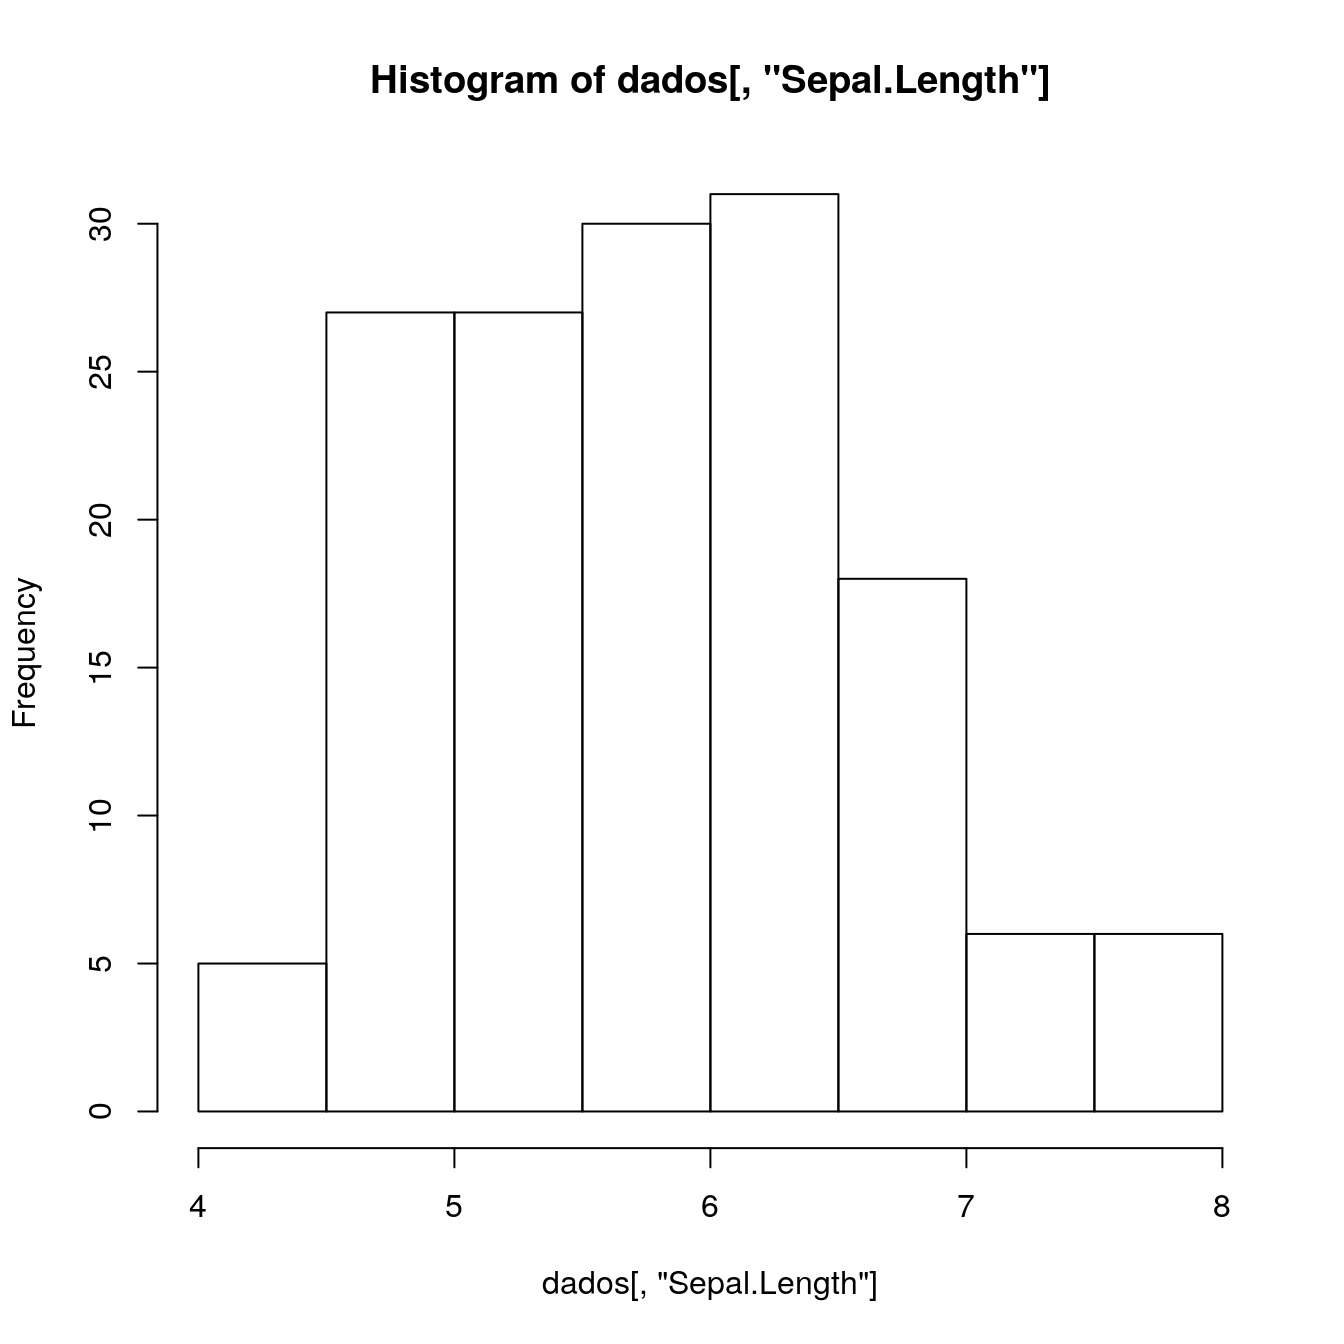
\includegraphics{introducao-ao-r_files/figure-latex/unnamed-chunk-10-1.pdf}

\begin{center}\rule{0.5\linewidth}{0.5pt}\end{center}

\textbf{\emph{Tarefa.}} \emph{No painel inferior direito do RStudio, acesse a aba \emph{Packages} e encontre o pacote chamado \texttt{graphics}. Navegue pelo índice de funções do pacote \texttt{graphics} e escolha a função gráfica que mais chamar a sua atenção. Descreva o propósito dessa função e tente replicar os exemplos mostrados em sua página de ajuda.}

\begin{center}\rule{0.5\linewidth}{0.5pt}\end{center}

\begin{Shaded}
\begin{Highlighting}[]
\KeywordTok{hist}\NormalTok{(dados[, }\StringTok{"Sepal.Length"}\NormalTok{],}
     \DataTypeTok{main =} \StringTok{"Histograma"}\NormalTok{,}
     \DataTypeTok{xlab =} \StringTok{"Comprimento da sépala (cm)"}\NormalTok{,}
     \DataTypeTok{ylab =} \StringTok{"Frequência absoluta"}\NormalTok{,}
     \DataTypeTok{col =} \StringTok{"gray"}\NormalTok{)}
\KeywordTok{rug}\NormalTok{(dados[, }\StringTok{"Sepal.Length"}\NormalTok{], }\DataTypeTok{col =} \StringTok{"red"}\NormalTok{)}
\end{Highlighting}
\end{Shaded}

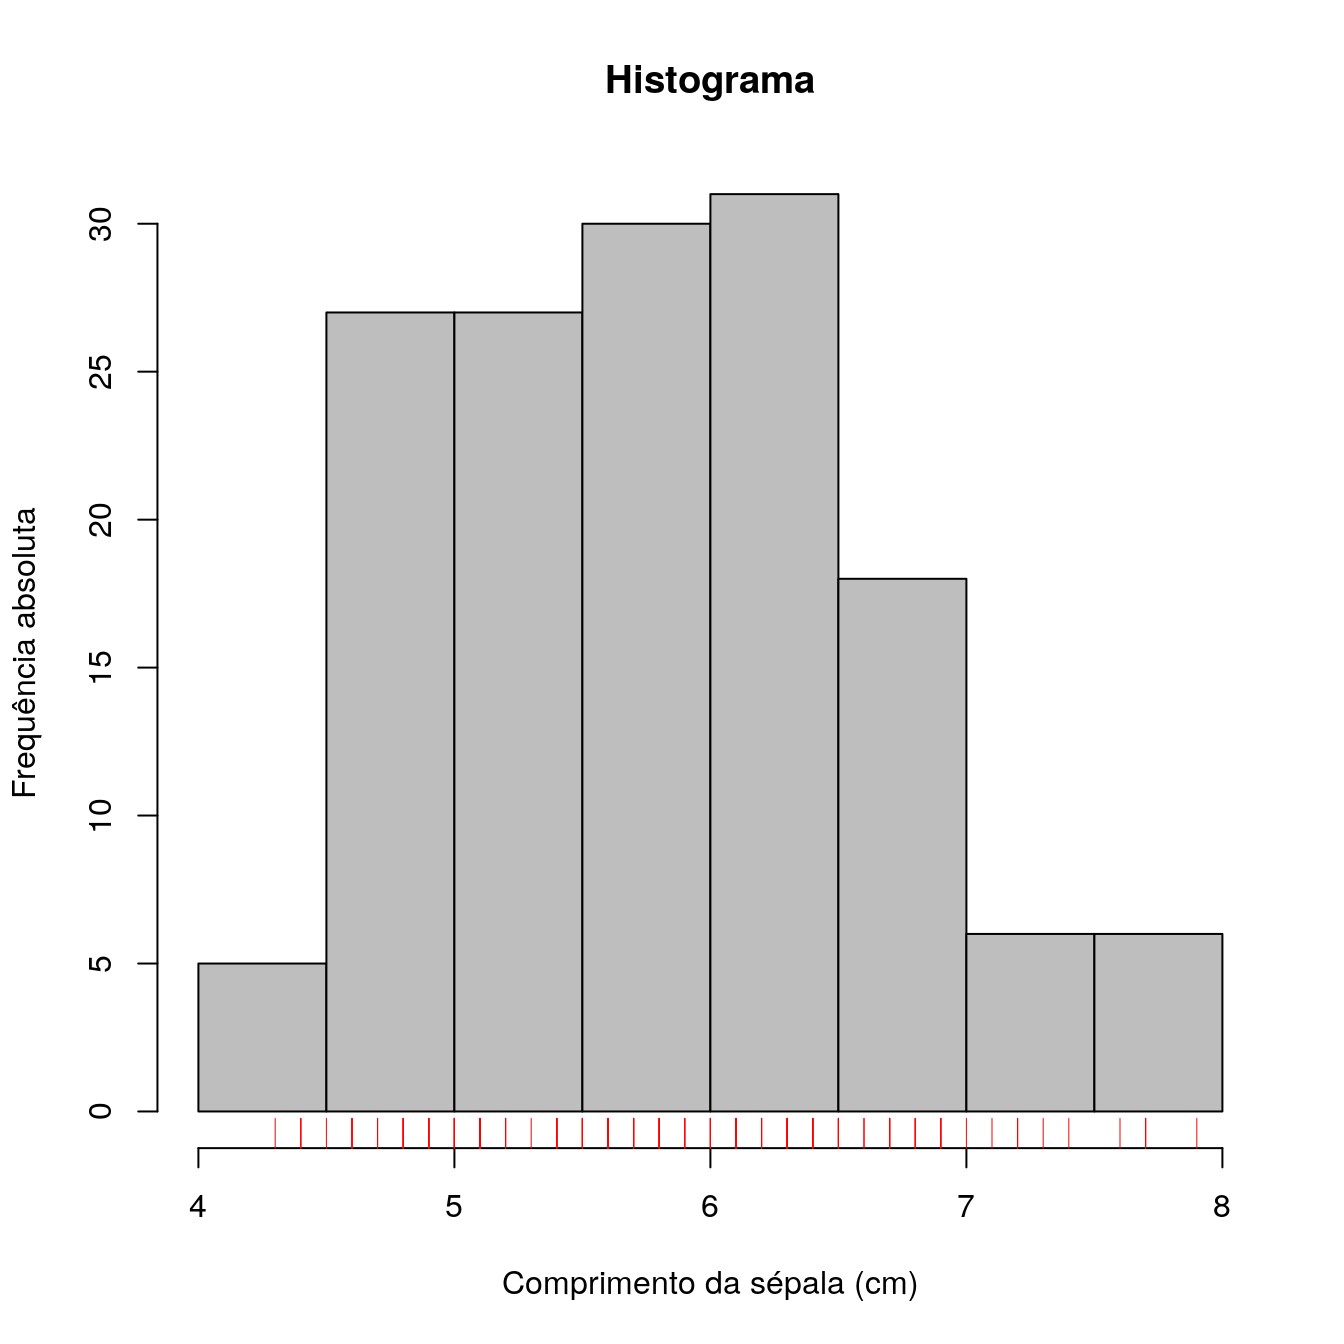
\includegraphics{introducao-ao-r_files/figure-latex/unnamed-chunk-11-1.pdf}

\begin{Shaded}
\begin{Highlighting}[]
\KeywordTok{dev.off}\NormalTok{()}
\KeywordTok{png}\NormalTok{(}\StringTok{"res/fig/histograma.png"}\NormalTok{)}
\KeywordTok{hist}\NormalTok{(dados[, }\StringTok{"Sepal.Length"}\NormalTok{],}
     \DataTypeTok{main =} \StringTok{"Histograma"}\NormalTok{,}
     \DataTypeTok{xlab =} \StringTok{"Comprimento da sépala (cm)"}\NormalTok{,}
     \DataTypeTok{ylab =} \StringTok{"Frequência absoluta"}\NormalTok{,}
     \DataTypeTok{panel.first =} \KeywordTok{grid}\NormalTok{(),}
     \DataTypeTok{col =} \StringTok{"gray"}\NormalTok{)}
\KeywordTok{rug}\NormalTok{(dados[, }\StringTok{"Sepal.Length"}\NormalTok{], }\DataTypeTok{col =} \StringTok{"red"}\NormalTok{)}
\KeywordTok{dev.off}\NormalTok{()}
\end{Highlighting}
\end{Shaded}

\hypertarget{gruxe1ficos-bivariados}{%
\chapter{Gráficos bivariados}\label{gruxe1ficos-bivariados}}

\begin{Shaded}
\begin{Highlighting}[]
\NormalTok{dados <-}\StringTok{ }\KeywordTok{read.table}\NormalTok{(}\StringTok{"data/iris.csv"}\NormalTok{, }\DataTypeTok{dec =} \StringTok{","}\NormalTok{, }\DataTypeTok{header =} \OtherTok{TRUE}\NormalTok{)}
\KeywordTok{str}\NormalTok{(dados)}
\end{Highlighting}
\end{Shaded}

\begin{verbatim}
## 'data.frame':    150 obs. of  5 variables:
##  $ Sepal.Length: num  5.1 4.9 4.7 4.6 5 5.4 4.6 5 4.4 4.9 ...
##  $ Sepal.Width : num  3.5 3 3.2 3.1 3.6 3.9 3.4 3.4 2.9 3.1 ...
##  $ Petal.Length: num  1.4 1.4 1.3 1.5 1.4 1.7 1.4 1.5 1.4 1.5 ...
##  $ Petal.Width : num  0.2 0.2 0.2 0.2 0.2 0.4 0.3 0.2 0.2 0.1 ...
##  $ Species     : Factor w/ 3 levels "setosa","versicolor",..: 1 1 1 1 1 1 1 1 1 1 ...
\end{verbatim}

\begin{Shaded}
\begin{Highlighting}[]
\KeywordTok{plot}\NormalTok{(dados[, }\KeywordTok{c}\NormalTok{(}\StringTok{"Sepal.Length"}\NormalTok{, }\StringTok{"Petal.Length"}\NormalTok{)])}
\end{Highlighting}
\end{Shaded}

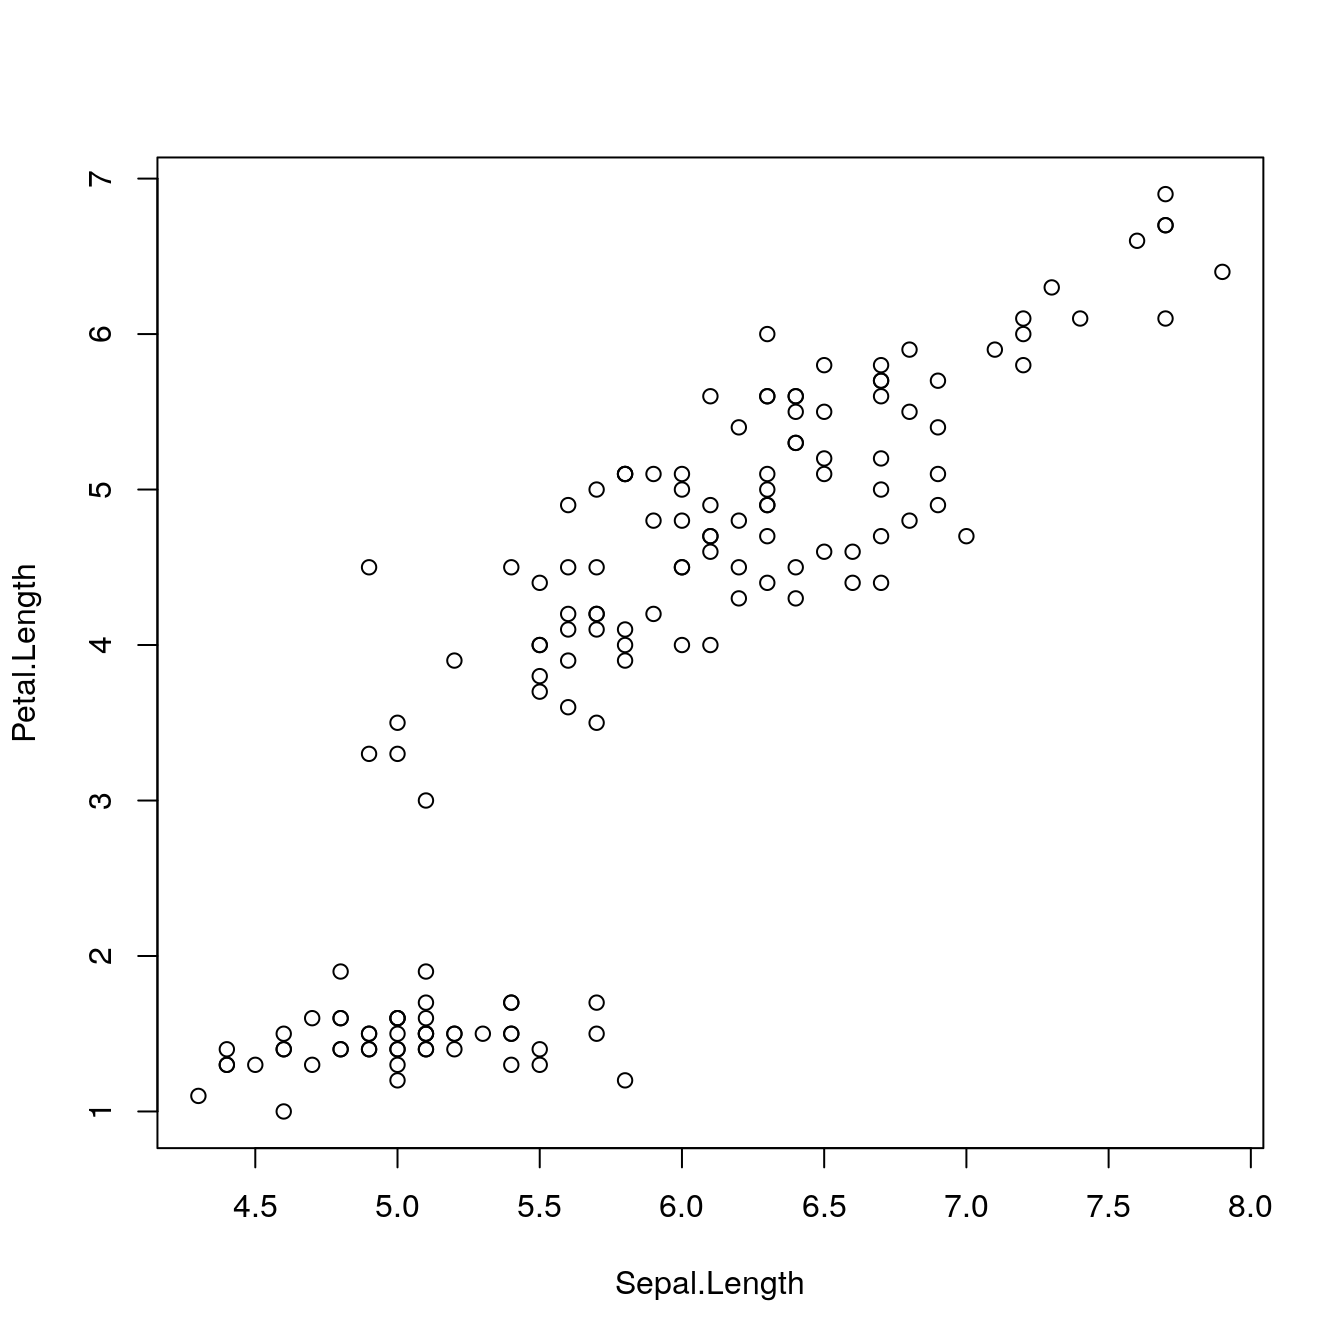
\includegraphics{introducao-ao-r_files/figure-latex/unnamed-chunk-14-1.pdf}

\begin{Shaded}
\begin{Highlighting}[]
\KeywordTok{plot}\NormalTok{(dados[, }\KeywordTok{c}\NormalTok{(}\StringTok{"Sepal.Length"}\NormalTok{, }\StringTok{"Petal.Length"}\NormalTok{)],}
     \DataTypeTok{xlab =} \StringTok{"Comprimento da sépala (cm)"}\NormalTok{,}
     \DataTypeTok{ylab =} \StringTok{"Comprimento da pétala (cm)"}\NormalTok{,}
     \DataTypeTok{xlim =} \KeywordTok{c}\NormalTok{(}\DecValTok{1}\NormalTok{, }\DecValTok{8}\NormalTok{), }\DataTypeTok{ylim =} \KeywordTok{c}\NormalTok{(}\DecValTok{1}\NormalTok{, }\DecValTok{8}\NormalTok{), }\DataTypeTok{pch =} \DecValTok{20}\NormalTok{,}
     \DataTypeTok{panel.first =} \KeywordTok{grid}\NormalTok{(), }\DataTypeTok{col =}\NormalTok{ dados[, }\StringTok{"Species"}\NormalTok{])}
\KeywordTok{abline}\NormalTok{(}\DataTypeTok{a =} \DecValTok{0}\NormalTok{, }\DataTypeTok{b =} \DecValTok{1}\NormalTok{, }\DataTypeTok{col =} \StringTok{"red"}\NormalTok{, }\DataTypeTok{lty =} \StringTok{"dashed"}\NormalTok{)}
\KeywordTok{legend}\NormalTok{(}\DataTypeTok{x =} \DecValTok{1}\NormalTok{, }\DataTypeTok{y =} \DecValTok{8}\NormalTok{, }\DataTypeTok{legend =} \KeywordTok{levels}\NormalTok{(dados[, }\StringTok{"Species"}\NormalTok{]), }
       \DataTypeTok{col =} \DecValTok{1}\OperatorTok{:}\DecValTok{3}\NormalTok{, }\DataTypeTok{pch =} \DecValTok{20}\NormalTok{, )}
\end{Highlighting}
\end{Shaded}

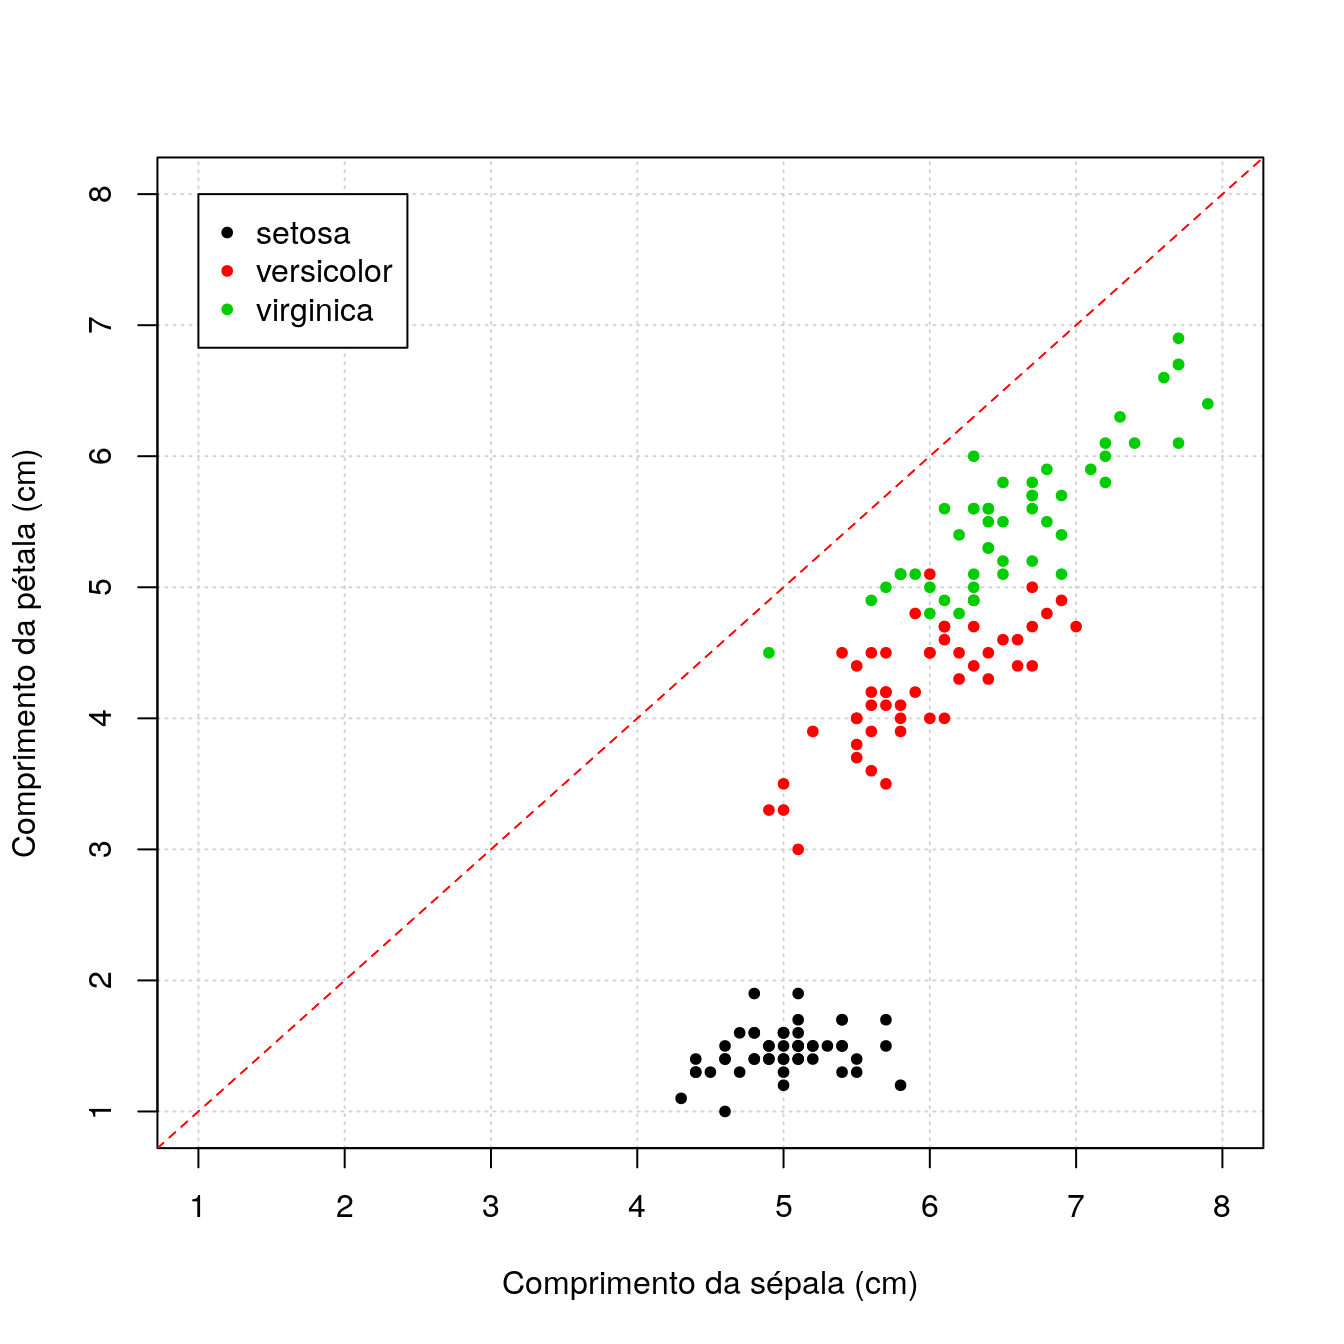
\includegraphics{introducao-ao-r_files/figure-latex/unnamed-chunk-15-1.pdf}

  \bibliography{book.bib,packages.bib}

\end{document}
